\documentclass[11pt]{article}

\usepackage{fullpage}
\usepackage{graphicx}
\usepackage{amsmath}
\usepackage{amssymb}
\usepackage{amsthm}
\usepackage{fancyvrb}

\parindent0in
\pagestyle{plain}
\thispagestyle{plain}


%% UPDATE MACRO DEFINITIONS %%
\newcommand{\myname}{Nguyen Quang Hao Tran - c3409773}
\newcommand{\assignment}{Python Web Socket Assignment}
\newcommand{\duedate}{October 18, 2024}

%% DO NOT CHANGE ANYTHING BELOW THIS LINE %%

\begin{document}
	
	\textbf{University of Newcastle}\hfill\textbf{\myname}\\[0.01in]
	\textbf{ELEC3500 -- Telecommunication Network}\hfill\textbf{\assignment}\\[0.01in]
	\textbf{Prof.\ Duy Ngo}\hfill\textbf{\duedate}\\
	\smallskip\hrule\bigskip
	
	\section{Questions}
	\begin{enumerate}
		\item \textbf{Considering the functionality of this simple proxy server, identify and discuss at least three significant limitations of your proxy server. (6 Marks)}
			\begin{itemize}
				\item \textbf{The server does not handle any request other than GET requests}\\
				In this sever implementation, the sever accept GET request. The GET method is used to get data from the server. Those data could be webpage (html file), image, video, CSS file, JavaScript file, etc. The GET reqest does not change state of any resources on the server.\\
				The problem in this server in this server implementation is that the server does not andle other request such as POST, DELETE, PUT, etc.
					\begin{itemize}
						\item POST request: The POST method is used to send data to the server. The data in HTTP POST method is stored int he request body of the HTTP request.
						\item DELETE request: The DELETE method is used to remove a resource on the server.
						\item PUT request: The PUT method is to replace existing resources on the server
					\end{itemize}
				The absence of other request method will limit the functionality of the sever. The server will not be able to perform more advanced task such as submit username and password.\\
				
				\item \textbf{The caching mechanism in this implemetation is too simple}\\
				In this proxy server implementation, all loaded files are stored in a cached folder. There are no expiration of the cache content or updates function. This could lead to user getting outdated content.\\
				
				\item \textbf{The sever is single threaded, which significantly slow down sever response} \\
				In this implementaion, we can know the server is single threaded by seeing the flow of the server. After accept a connection, the server immediately call the \texttt{handle\_client(cliSock)}. The \texttt{handle\_client} method only handle one client connection and process the request fully before accepting another client response. Therefore, the other client wants to connect has to wait for the previous one to complete because they can process. This attempt significantly slow down the speed of the server. Loading a simple webpage such as the ... could take more than 10 seconds.\\
			\end{itemize}
		
		\item \textbf{How could you implement potential improvements into this script to overcome these limitations? A flowchart or pseudocode may help to illustrate your answer. (6 marks)}\\
			\begin{itemize}
				\item \textbf{Lacking HTTP request handle} \\
					I would build POST request in the \texttt{handle\_client() method} that would allow user to input data to send to the server.\\
					\begin{center}
						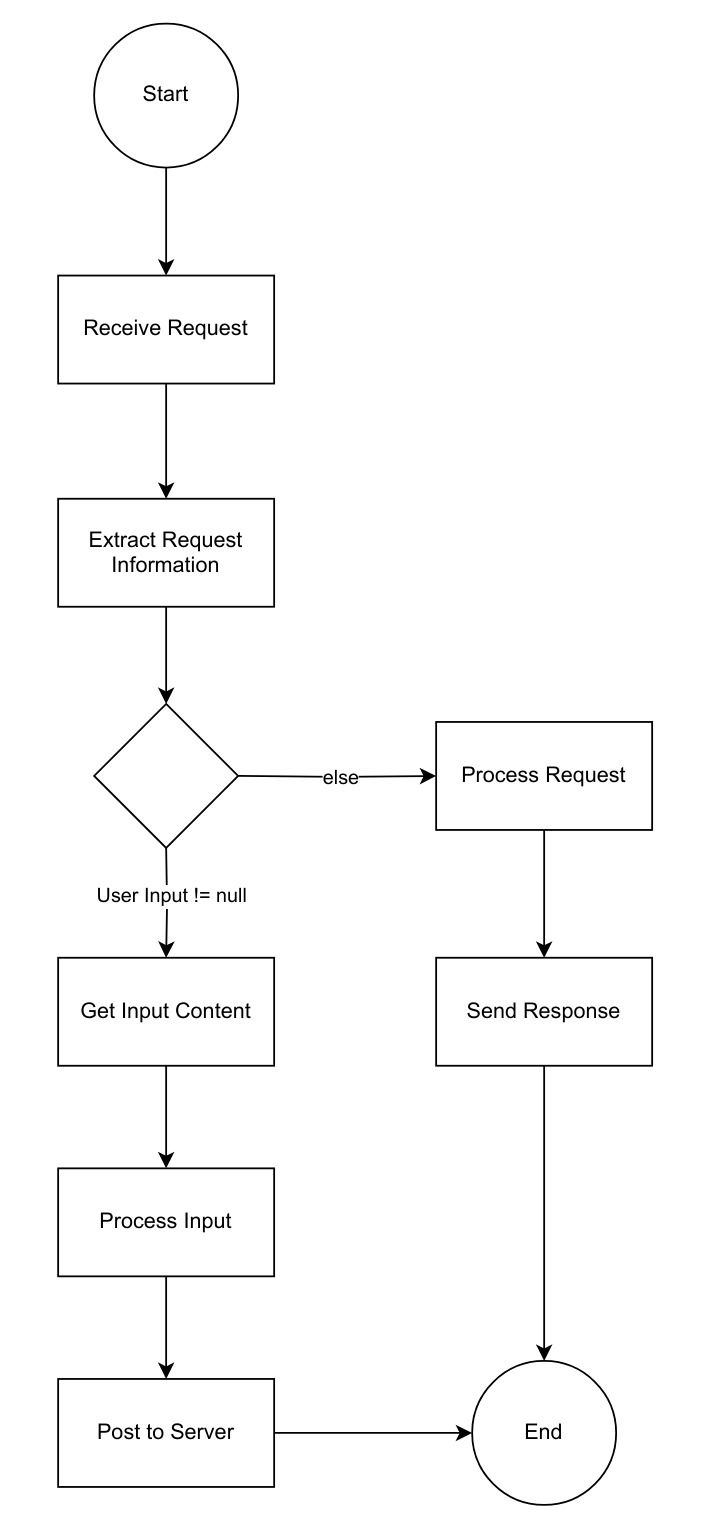
\includegraphics[scale=0.4]{post.png}
					\end{center}
				\pagebreak
				  
				\item \textbf{Simple Caching}\\
					A solution for this is to add a mechanism to auto delete the cache files after a specific amount of time. It could be somewhere 5 to 10 minutes
				\item \textbf{Single Thread Implementation}\\
					\begin{center}
						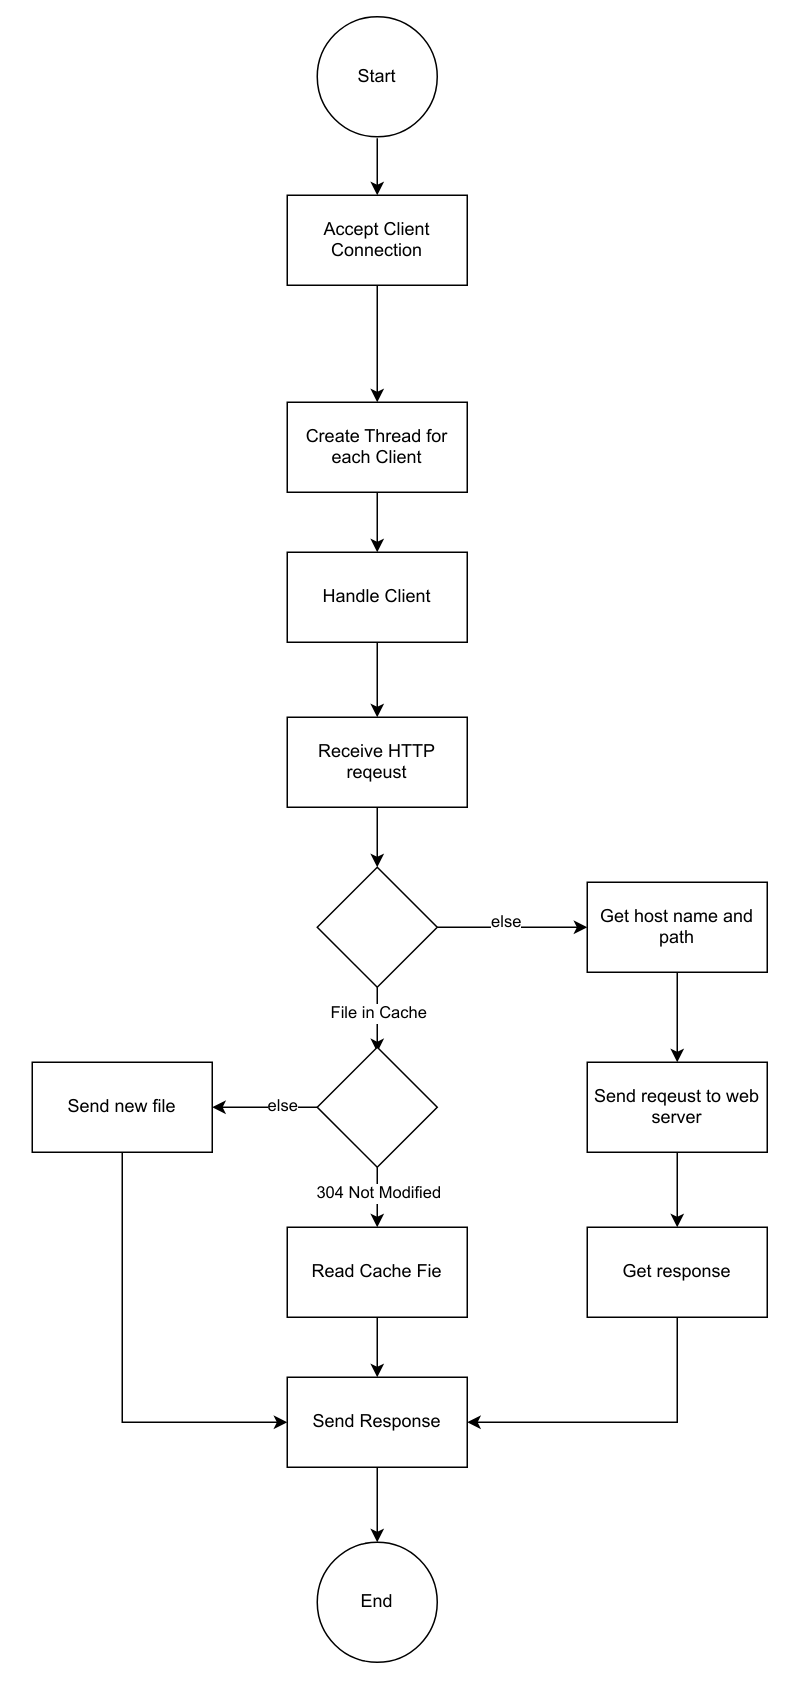
\includegraphics[scale=0.3]{multi_thread.png}
					\end{center}  
			\end{itemize}
		\item \textbf{Is the proxy server using UDP or TCP sockets? How can you tell? What other protocols are involved?(2 marks)}\\
		To know if the proxy server is using a UDP or TCP socket, I looked at the initialization of the socket server: \texttt{servSock = socket(AF\_INET, SOCK\_STREAM)}. The socket is using \texttt{SOCK\_STREAM} as the argument, which is used for a TCP connection. If it were to be UDP, the argument should be \texttt{SOCK\_DGRAM}.
		
		Other Protocols Involved:
		
			\begin{itemize}
				\item HTTP (Hypertext Transfer Protocol): The proxy server is fetching web pages, which are delivered using HTTP. The proxy forwards HTTP `GET` requests to the web server and receives HTTP responses.
				\item DNS (Domain Name System): DNS may be involved implicitly if the URL contains a domain name that needs to be resolved to an IP address before the proxy can communicate with the web server.
			\end{itemize}
		So, the proxy server uses TCP sockets, and the protocols involved are TCP, HTTP, and possibly DNS.
		
		\item \textbf{In this question, you will put together much of what you have learned about Internet protocols. Suppose you buy a brand new computer, connect it to Ethernet, and want to download a Web page. What are all the protocol steps that take place, starting from powering on your PC to getting the Web page? Assume there is nothing in our DNS or browser caches when you power on your PC. (Hint: the steps include the use of Ethernet, DHCP, ARP, DNS, TCP, and HTTP protocols.) Explicitly indicate in your steps how you obtain the IP and MAC addresses of a gateway router. (6 marks)}\\
		
		The first step after starting the computer is to use the Ethernet to use Dynamic Host Configuration Protocol (DHCP), a network management protocol, to configure devices on the Internet Protocol (IP) network. DHCP will provide the device with a unique IP address and also help us to get all neighbor routers' IP. Next, The computer will use Address Resolution Protocol (ARP) to map an IP address to a device's Media Access Control (MAC) address within a local network. The Domain Name System (DNS) is also obtained in this stage. When the user wants to fetch a webpage, the DNS will be used to find the IP address of the web page. Finally, the computer will send a Hypertext Transfer Protocol (HTTP) request to open the page in a browser. The server will then respond with the content and display it in the browser. The Transmission Control Protocol (TCP), IP datagram, and Ethernet frame are the result of the division and encapsulation of this request. The packet then goes through all interfaces to get to the destination.\\
	\end{enumerate}
\end{document}  